\section{RNA Basics}
\begin{frame}{Was ist RNA?}
	\begin{itemize}
			\item RNA besteht aus einer Aneinandereihung von Nukleotiden
			\item Die Nukleotide bestehen aus einer Base, Ribose und einem Phosphat.
			\item Es gibt vier verschiedene mögliche Basen Adenin (A), Guanin (G), Cytosin (C) und Uracil (U)
			\item Die Kombination aus Ribose und Phosphat wird auch als Backbone bezeichnet
			\item RNA ist zum Beispiel bei der Herstellungen von Proteinen beiteiligt und liefert dabei genetische Informationen in Form von mRNA.
	\end{itemize}
\end{frame}

\begin{frame}{RNA - Primärstruktur}
\vspace*{\fill}
\begin{figure}
	
\includegraphics[width=1\textwidth]{imgs/pst.png}
\end{figure}	
\vspace*{\fill}
\end{frame}

\begin{frame}{RNA - Sekundärstruktur}
\vspace*{\fill}
\begin{figure}
	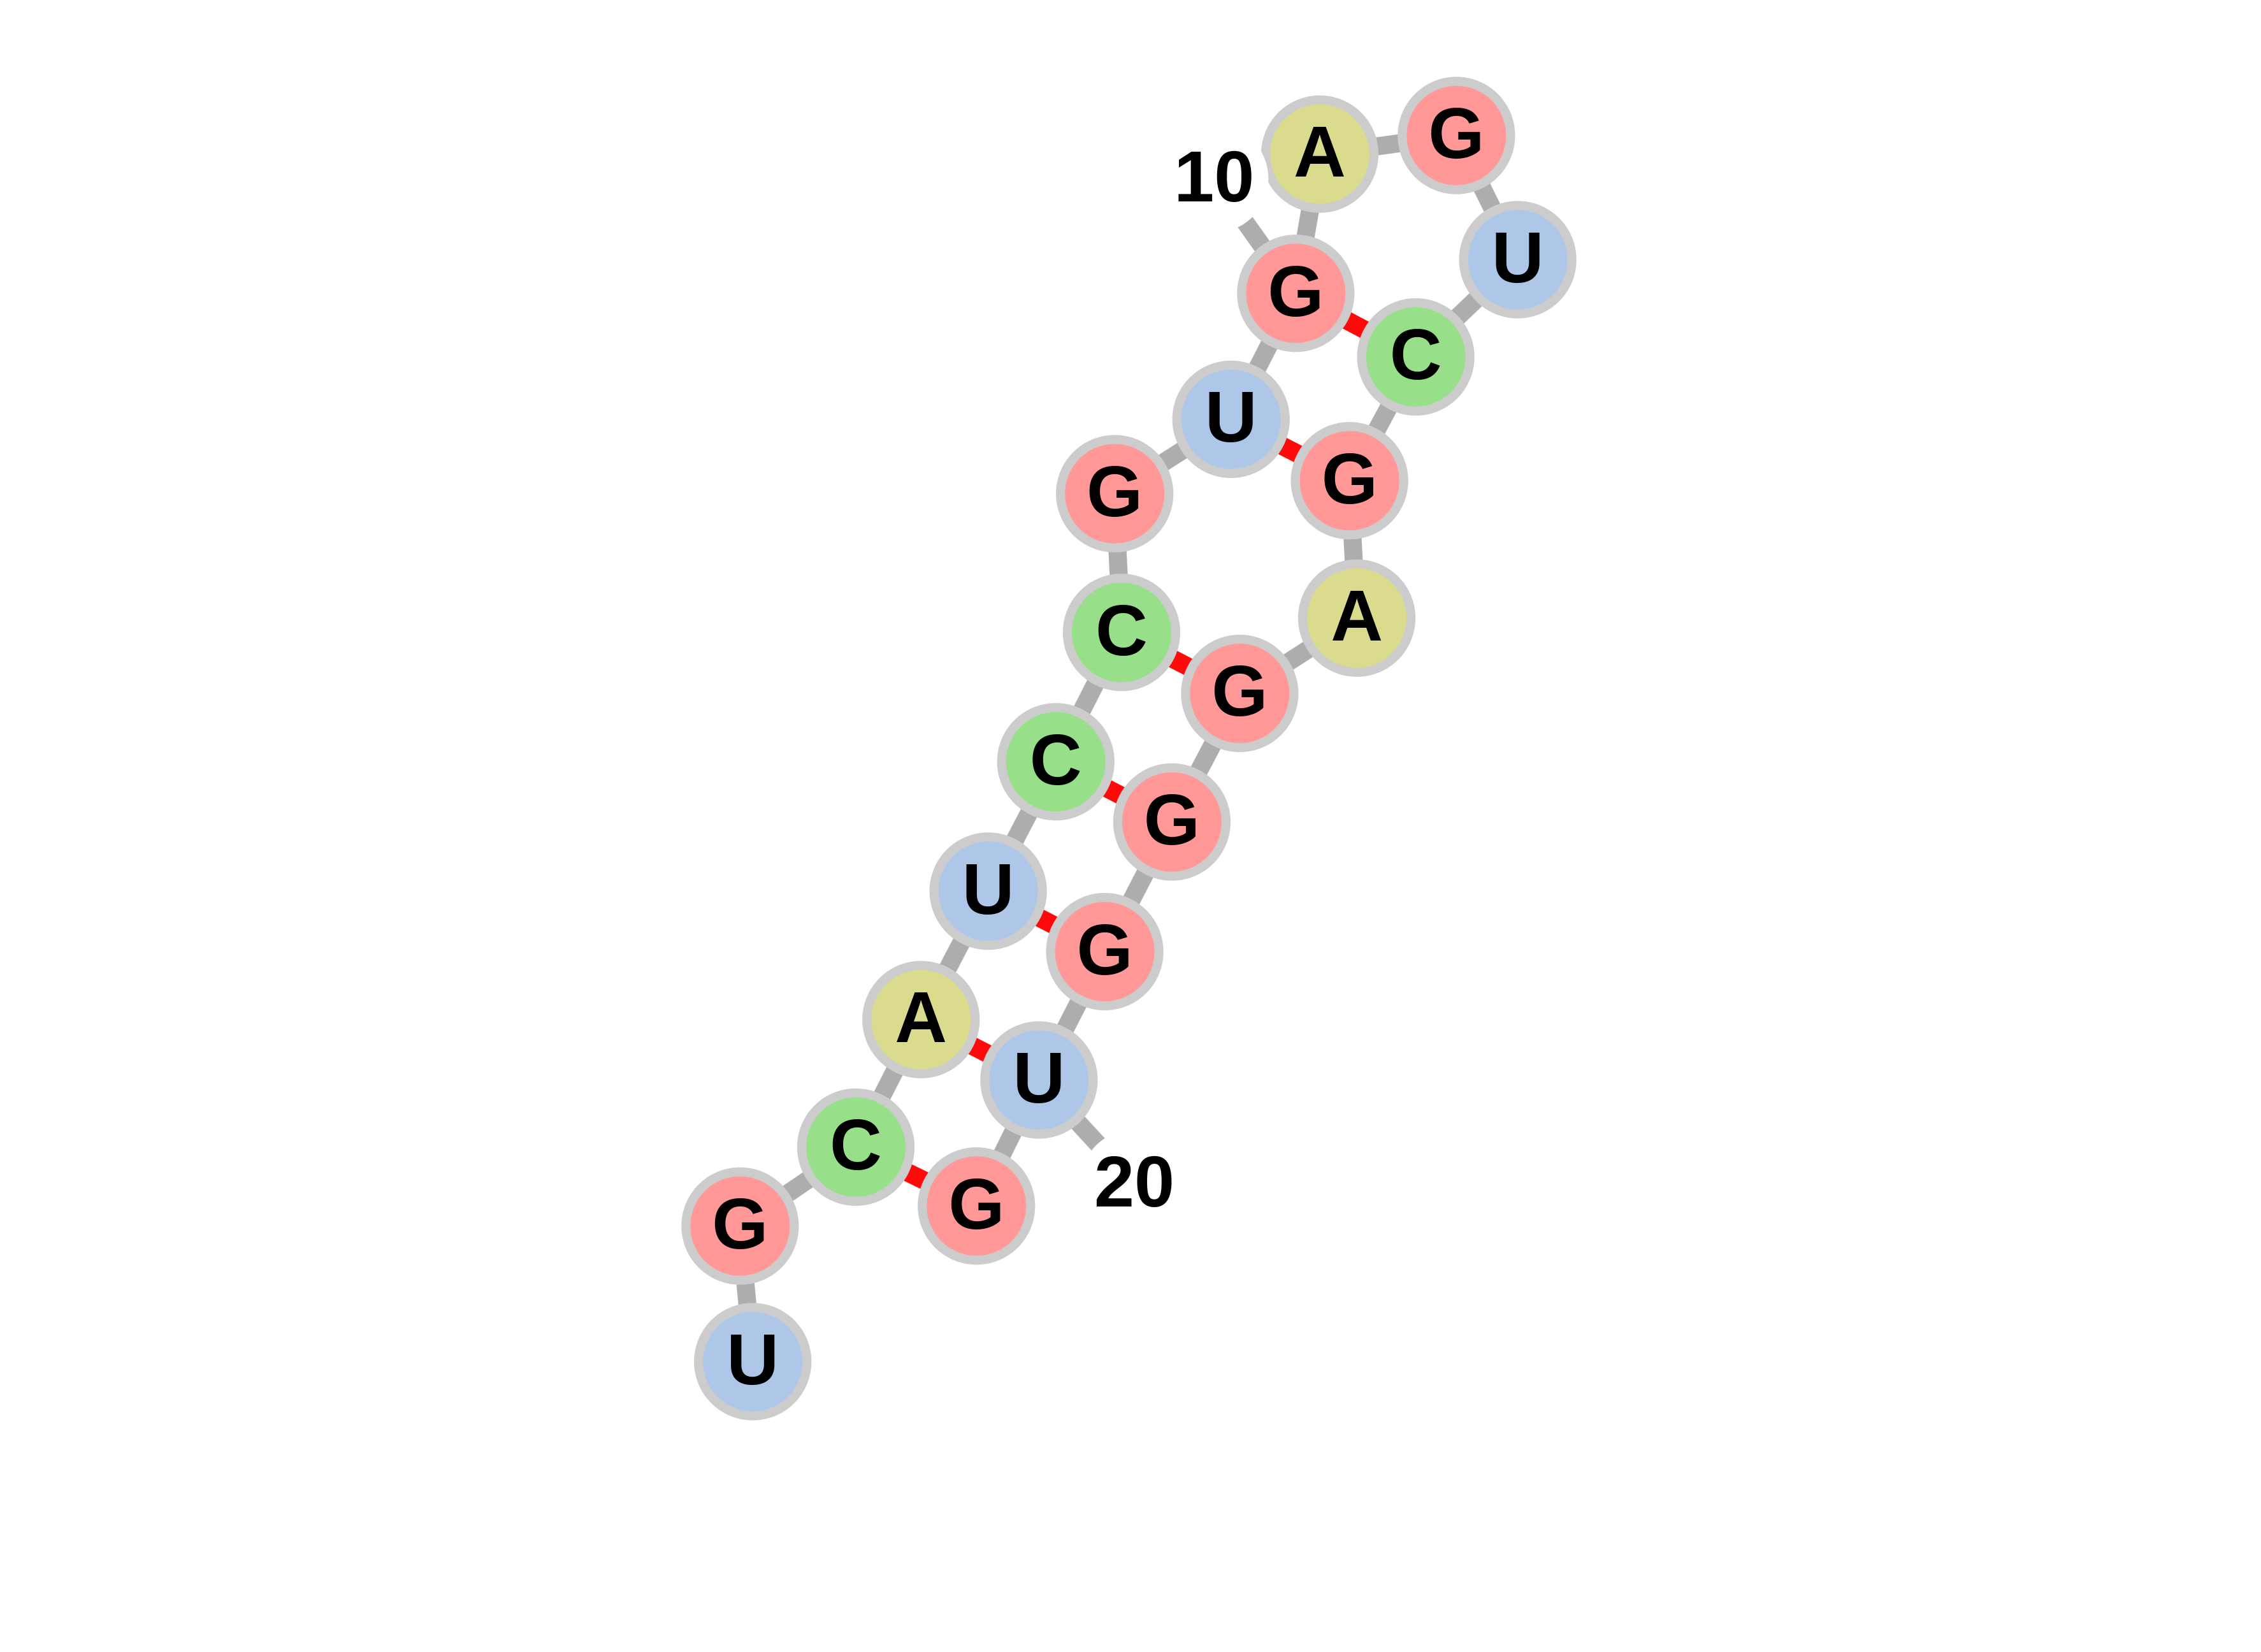
\includegraphics[width=0.7\textwidth]{imgs/sst.png}
\end{figure}	
\vspace*{\fill}
\end{frame}

\begin{frame}{RNA - Tertiärstruktur}
\vspace*{\fill}
\begin{figure}
	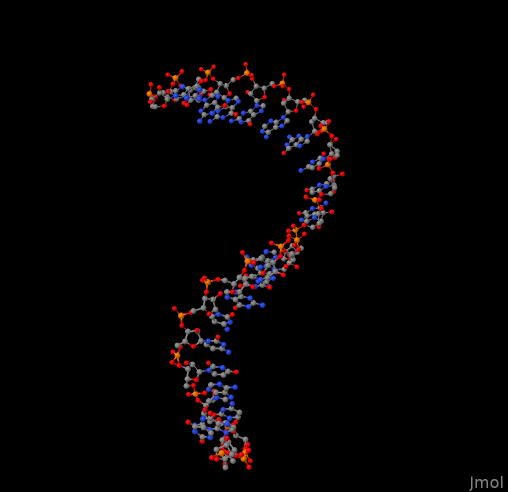
\includegraphics[width=.4\textwidth]{imgs/tst.png}
\end{figure}	
\vspace*{\fill}
\end{frame}

\begin{frame}{Warum braucht man die Tertiärstruktur?}
	Über die Tertiärstruktur erfährt man vieles über die Eigenschaften der RNA wie zum Beispiel
	\begin{itemize}
			\item Funktion
			\item Ineraktion mit anderen Molekülen
			\item Stabilität
	\end{itemize}
	\vspace{.5cm}
	Die Tertiärstruktur hat einige praktische Anwendungen:
	\begin{itemize}
			\item Biologische Prozesse verstehen
			\item Design eigener RNA die gewünschte Funktion hat (z. B. RNA-Impfstoff)
	\end{itemize}

\end{frame}
